\section{Test set and cross-validation}
\begin{frame}{Mục lục}
	\tableofcontents[currentsection]
\end{frame}

\begin{frame}{Test set and cross-validation}
	Trong quá trình train và test cho text classfication, ta sẽ có 3 tập: 
	\begin{itemize}
		\item \textbf{Training set} là tập dùng để huấn luyện mô hình.
		\item \textbf{Development test set hay devset} là tập dùng để điều chỉnh tham số (tune parameters)
		\item \textbf{Test set} là tập dùng để đánh giá khả năng tổng quát hóa của mô hình ở bước cuối cùng.
	\end{itemize}
\end{frame}

\begin{frame}{Test set and cross-validation}
	\begin{itemize}
		\item Trong quá trình sử dụng tập devtest, để tránh việc \textbf{quá khớp} (overfit) với tập test set, chúng ta thường hay \textbf{cố định} các tập train, dev, test.
		\item Điều này dẫn tới câu chuyện nếu muốn có nhiều dữ liệu để train thì tập dev hoặc test sẽ \textbf{không đủ lớn} để làm tập đại diện.
		\item Câu hỏi đặt ra là liệu có cách nào để sử dụng toàn bộ dữ liệu để huấn luyện (train) mà vẫn muốn sử dụng tất cả để kiểm tra (test) hay không? 
		\pause
		$\Rightarrow$ Sử dụng \textbf{cross-validation}.
	\end{itemize}
\end{frame}

\begin{frame}{Test set and cross-validation}
	\begin{itemize}
		\item Với một giá trị $k$ ta chọn trước, ta chia tập dữ liệu thành $k$ một tập con gọi là \textbf{folds}. 
		\item Bây giờ, khi ta chọn một trong $k$ tập folds làm tập test set thì ta có thể huấn luyện trên $k-1$ tập còn lại và tính \textbf{error rate} (tỉ lệ lỗi) trên tập test set. 
		\item Lặp lại với $k-1$ tập folds còn lại, ta sẽ tính \textbf{average error rate} (tỉ lệ lỗi trung bình) thông qua trung bình error rate trong $k$ lần chạy.
	\end{itemize}
\end{frame}

\begin{frame}{Test set and cross-validation}
	\begin{itemize}
	\item Tuy nhiên, cross-validation cũng có một hạn chế là toàn bộ dữ liệu đều sẽ có lúc được dùng để test, nên ta không thể thoải mái nhìn vào dữ liệu để phân tích feature như trong nhiều bài toán NLP khác.
	
	\item Trên thực tế, người ta thường giữ một test set cố định và chưa đụng tới, còn dùng cross-validation bên trong training set để điều chỉnh tham số và chọn mô hình.
	\end{itemize}
	
\end{frame}

\begin{frame}{Test set and cross-validation}
	\begin{figure}
		\centering
		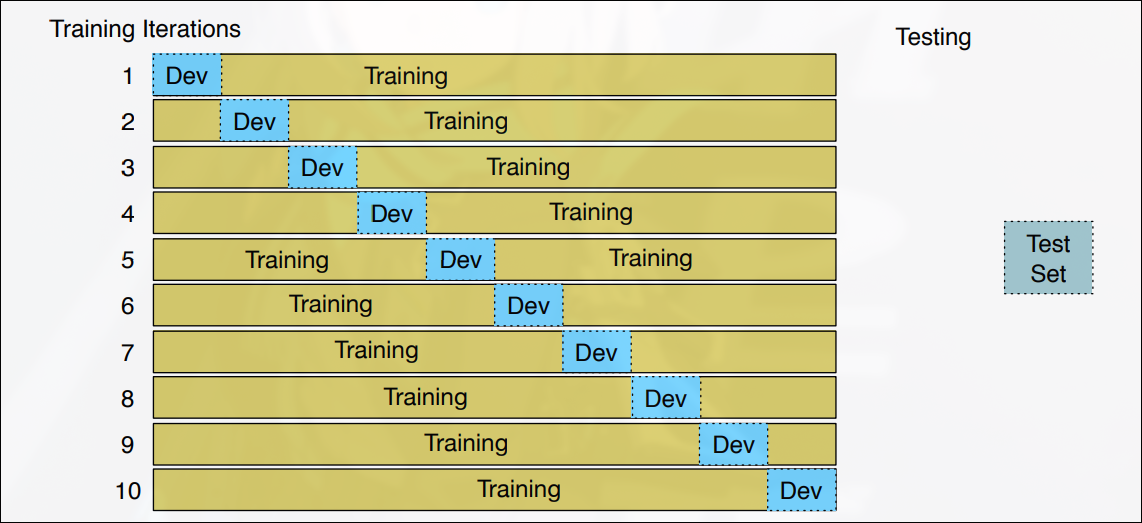
\includegraphics[width=1\linewidth]{cross-validation}
	\end{figure}
\end{frame}